\documentclass[a4paper]{article}
\usepackage{graphicx}
\usepackage{xcolor}
\usepackage{url}
\usepackage{outlines}
\usepackage{listings}
\usepackage{fontspec}
\lstset{basicstyle=\ttfamily,
	showstringspaces=false,
	commentstyle=\color{blue},
	keywordstyle=\color{pink}
}
\lstset{emph={
	EXPOSE,RUN,FROM,CMD,nc,tcp,udp,http,docker},emphstyle=\color{purple}
}
% \renewcommand{\\}{\hfill \break}
\usepackage{fancyhdr}
\usepackage{geometry}
\geometry{
	a4paper,
	total={170mm,257mm},
	left=20mm,
	top=20mm,
	bottom=39mm,
}

\setlength{\headheight}{82.70538pt}

\fancypagestyle{oida}{
	\fancyhf{}
	\fancyhead[L]{\fontsize{7.5}{7.5}htl donaustadt\\ Donaustadtstraße 45\\
		1220 Wien\\~\\ Abteilung: Informationstechnologie\\ 
	Schwerpunkt: Netzwerktechnik}
	\fancyhead[R]{
\includegraphics[scale=0.45]{images/logo.png}}

	\fancyfoot[L]{\today}
	\fancyfoot[C]{\jobname}
	\fancyfoot[R]{Page: \thepage}
}

\begin{document}
\bibliographystyle{plain}
\pagestyle{oida}
\section*{Thema}
\par\noindent\rule{\textwidth}{0.4pt}

Laboratory protocol
GNU/Linux - Setting up a multi-user environment

\begin{figure}[h]
	
\includegraphics[scale=0.3]{images/mika.jpeg}
	\caption{Grouplogo}
\end{figure}

\vspace*{\fill}
Subject:	ITSI|ZIVK

Class:	3AHITN

Name:	Stefan Fürst, Marcel Raichle

Groupname/number: Dumm und Dümmer/7

Supervisor: 	ZIVK

Exercise dates:	25.10.2024, 1.11.2024, 3.11.2024, 6.11.2024

Submission date: 6.11.2024


\newpage
\tableofcontents

\newpage

\section{Task definition}

Setting up a headless Linux installation with multiple users, adding them to a group, and setting permissions over a directory structure. You will also need to set up an ssh server for which you will need to set up key pair authentication.


\section{Summary}

To accomplish this, we set up a Docker image that does all the necessary setup so that the container can be rebuilt at any time for easier testing instead of using a heavier vm. To make it easier to rebuild and restart the container, we wrote a shell script to the source so that we had aliases for all the commands. We used the Ubuntu Docker image as a base, installed the required packages since the image comes with a minimal amount of packages, and used \texttt{useradd, chmod, chown, chgrp, su} to add users, change file ownership, permissions and test. Finally, for the ssh part, the service was set up and configured appropriately. We did everything that made sense in the Dockerfile file to make it reproducible. 


\newpage

\section{Exercise Execution}

\subsection{Creating the Container}

I decided to write my own dockerfile for this, which is a text file that describes the commands needed to create the desired image. Lets walk through how to create an image for the first task. \\
We start by using the \texttt{FROM} keyword to specify the base image \cite{docker-glossary} from which we are starting.
\\
\texttt{FROM ubuntu:latest} \\
I chose the ubuntu image \cite{ubuntu} and used the \texttt{latest} tag, which points to the latest LTS release.\\
However, if we were to build, start, and execute in the container, we would not be able to do it because it would immediately showdown since nothing is running. \\
To mitigate this, we add \texttt{CMD tail -F /dev/null} to the end of our Dockerfile. The \texttt{tail} command prints the last 10 lines of a file and the \texttt{-F} argument stands for follow, so it will run forever and print the last 10 lines of a given file.\cite{tail} I used the file \texttt{/dev/null}, which is a virtual device, so any data written to it will disappear. \cite{devnull} So we are essentially reading an empty file forever to keep the container up. \\

If we now run the following commands to build the image, run the container and get a shell in it.
\begin{lstlisting}[language=bash]
#build the image
docker buildx build -t image-name .
#run the container
docker run -d --name container-name 
#exec into the container (get a shell in it)
docker exec -it container-name /bin/bash
\end{lstlisting}
To make to commands less work to type, i like to make a shell script that i can source to have aliases for it like this.
\begin{lstlisting}[language=bash]
#!/bin/sh
alias relaunch="sudo sh -c 'docker stop itsi &&\
      docker rm itsi &&\
      docker buildx build -t itsi:latest . &&\
      docker run -d -p 38452:38452 --name itsi itsi:latest &&\
      docker exec -it itsi /bin/bash'"
alias rebuild="sudo sh -c 'docker buildx build -t itsi:latest . &&\
      docker run -d -p 38452:38452 --name itsi itsi:latest &&\
      docker exec -it itsi /bin/bash'"
alias stop="sudo sh -c 'docker stop itsi && docker rm itsi'"
\end{lstlisting}
Now we are in the container, but it does not have any of the required packages installed that are needed for this exercise. They can be installed in the container now, which would defeat the whole purpose of building an image, so we use the \texttt{RUN} keyword in our dockerfile along with the desired command to run it when the image is built, so that the packages are installed as soon as you spin up the container:
\begin{lstlisting}[language=bash]
RUN apt update 
RUN apt upgrade -y
RUN apt install iproute2 iputils-ping zsh net-tools vim -y
\end{lstlisting}
\newpage
\subsection{Testing Connectivity}
Now we can finally test the connectivity since we have the \texttt{iputils-ping} package installed. Everything works out of the box using the default bridge \cite{Docker-bridge}

\begin{figure}[h]
	\centering
	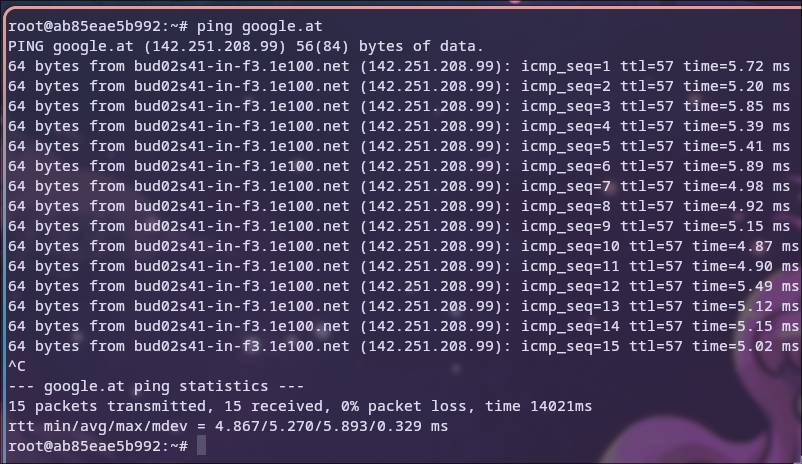
\includegraphics[scale=0.3]{images/ping_internet.png}
	\caption{Ping to the Internet}
\end{figure}
\begin{figure}[h]
	\centering
	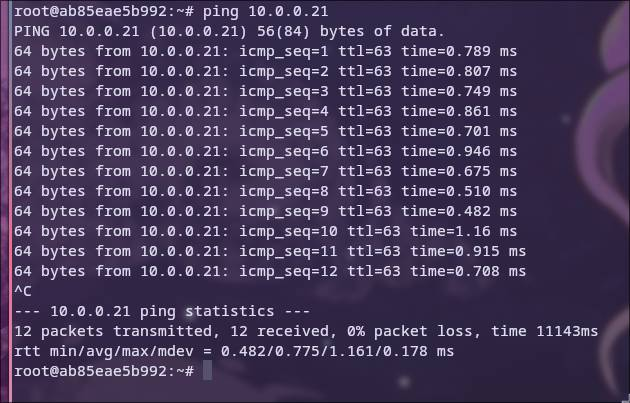
\includegraphics[scale=0.3]{images/ping_lokal.png}
	\caption{Ping the local machine}
\end{figure}
\newpage
\subsubsection {It works, but why?}

If we inspect our container using \texttt{docker inspect container-name}, we see that its IP is different from that of the lan.

\begin{figure}[h]
	\centering
	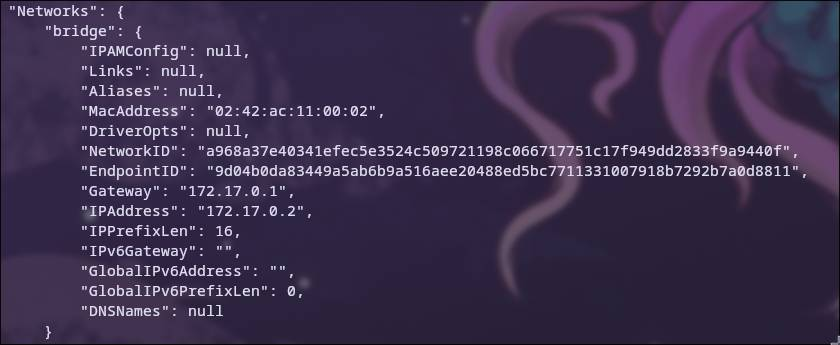
\includegraphics[scale=0.3]{images/docker_inspect_nw.png}
	\caption{docker inspect}
\end{figure}
This happens because when you install Docker, it creates a virtual interface \texttt{docker0} that is used as a network bridge to allow the container to communicate with the Internet and LAN. \cite{docker-networking-video}
\begin{figure}[h]
	\centering
	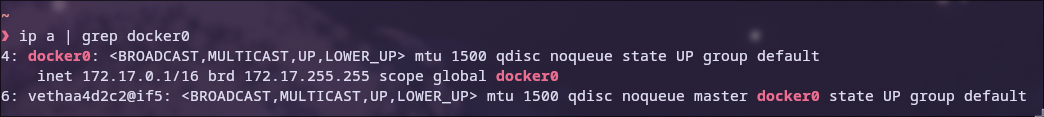
\includegraphics[scale=0.3]{images/ipadocker.png}
	\caption{ip a | grep docker0}
\end{figure}
There are other types of Docker networks, but they are not relevant for this exercise.\cite{docker-networking-video}

\newpage
\subsection{creating and managing users}

To add groups and users, use the commands \texttt{groupadd} and \texttt{useradd}.
To add the user, we add the following lines to our Dockerfile
\begin{lstlisting}[language=bash]
#creating the group
RUN groupadd -g 324 ram-Users 
#creating the users -u is used to set the groupid
RUN useradd -u 1024 ram-alois &&\
    useradd -u 1124 ram-berta &&\
    useradd -u 1224 ram-chris &&\
    useradd ram-fus &&\
    useradd ram-ram
#adding the users to the groups
RUN usermod -g ram-Users ram-alois &&\
    usermod -g ram-Users ram-berta
#settings chris's default shell to zsh
RUN usermod --shell /bin/zsh ram-chris 
\end{lstlisting}
\subsubsection{logging in as the users}

To log in as another user, use the \texttt{su} command.

\begin{figure}[h]
	\centering
	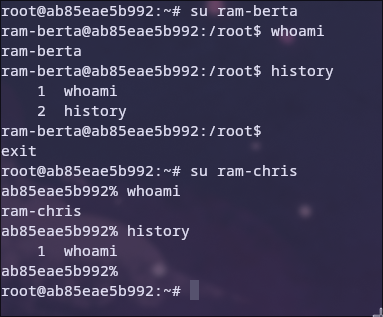
\includegraphics[scale=0.3]{images/logggingin.png}
	\caption{Login as Berta and Chris}
\end{figure}
Each user has their own history, which is stored in their home directory in either the \texttt{.bash\_history} or \texttt{.zsh\_history} file. You end the session with the \texttt{exit} command or by pressing \texttt{<C-d>}.
\subsection {Set directory privileges}
The directories are created with this command and the \texttt{-p} stands for parent and creates parent directories if needed. For example, \texttt{mkdir /test/test2} wouldn't work if you don't have \texttt{/test}, but using \texttt{mkdir -p} instead will create \texttt{/test} and \texttt{/test/test2}.
\begin{lstlisting}[language=bash]
RUN mkdir -p /data/fus &&\
    mkdir /data/fus/alois &&\
    mkdir /data/fus/berta &&\
    mkdir /data/fus/chris &&\
    mkdir /data/fus/public
\end{lstlisting}
Three tools are used to set the permission: \texttt{chrgrp}, \texttt{chown} and \texttt{chmod}. \\
First, we want everyone in the group to have access to the directory for which \texttt{chgrp -R ram-Users /data/fus/} is used with the \texttt{-R} argument, which means recursive \cite{perms,chgrp}.
\\To give everyone all the permissions in their own directory, we need to make them the owner of it using \texttt{chown -R username:groupname /data/fus/name-of-directory}.\cite{chown} \\
Now we can assign permissions to each directory using the \texttt{chmod}\cite{chmod} command. \\
To better understand the command, here is a breakdown of the options: \\ 
\begin{lstlisting}
u = user who owns the file
g = group -> everyone in the group of the owner
o = other -> everyone else
r = read
w = write
x = execute
+ adding permissions
- removing permissions
= setting permissions
\end{lstlisting} \cite{chmod}
Now, let us use this to set up the permissions accordingly
\begin{lstlisting}[language=bash]
#giving the [g]roup [r]ead and [w]write permissions for /data/fus
chmod g+rw /data/fus/
#giving the owner all permissions, the [g]roup only read [r]ead and none to [o]thers
chmod -R u+wrx,g=r,o= /data/fus/alois/
#same for berta
#giving the owner all permissions and none to the [g]roup and [o]thers
chmod -R u+wrx,g=,o= /data/fus/chris/ 
#giving the owner and [g]roup all permissions and none to [o]thers
chmod -R u+wrx,g+wrx,o=r /data/fus/public/
\end{lstlisting} \cite{chmod}
\begin{figure}[h]
	\centering
	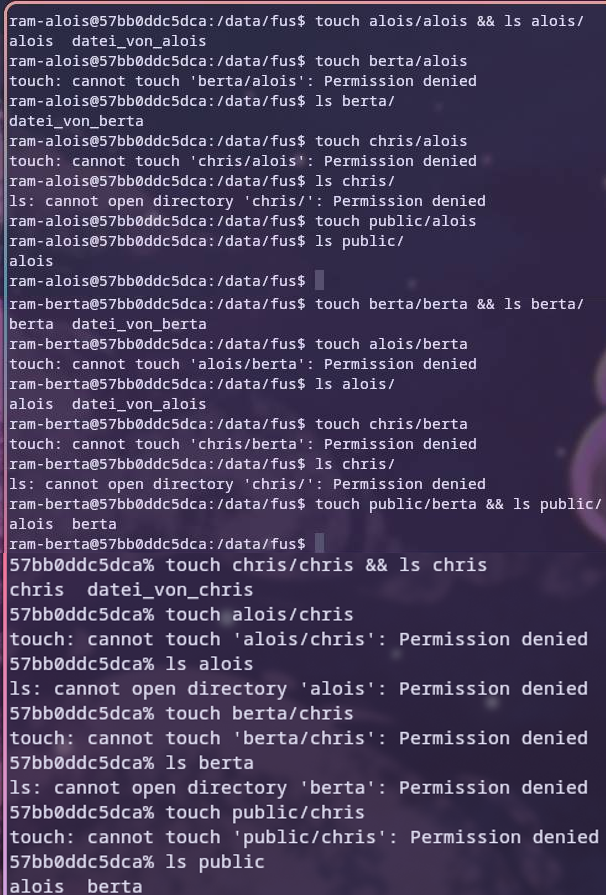
\includegraphics[scale=1.2]{images/testing_perms.png}
	\caption{Testing permissions}
\end{figure} \\
If we log in as the users, we can see that everything is working as intended.
\newpage
\subsection {setting up ssh}
The two new users required for this have already been created above in 3.3 \\
To set up an ssh server we need to install the package, if we just add \texttt{ssh} to our install command in the Dockerfile we find out that this command requires interactions to set the timezone we need to add these two extra lines to the Dockerfile.
\begin{lstlisting}[language=bash]
#setting the timezone
RUN ln -fs /usr/share/zoneinfo/Europe/Vienna /etc/localtime
#running the command without it beeing interactive
RUN DEBIAN_FRONTEND=noninteractive apt install -y tzdata ssh
\end{lstlisting}
Now ssh is installed, but it needs to be started, all we need to do is edit the last line of the file to start the service as well.
\begin{lstlisting}[language=bash]
#the default command from before
CMD tail -F /dev/null
#with starting ssh
CMD service ssh start && tail -F /dev/null
\end{lstlisting}
To find out what port the server is listening on for ssh, we use the netstat command that comes with the \texttt{net-tools} package that we installed earlier.
This is done with the command \texttt{netstat -tunlp | grep ssh}. The options of the command are explained below.
\begin{lstlisting}[language=bash]
-t show TCP ports
-u show UDP ports
-n show numerical addresses instead of resolving hosts
-l show only listening ports
-p show the PID of the listener's process
\end{lstlisting}\cite{netstat}
\begin{figure}[h]
	\centering
	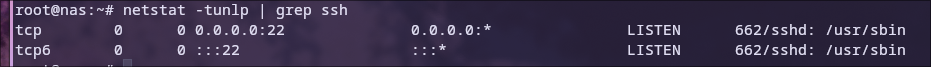
\includegraphics[scale=0.4]{images/netstatssh.png}
	\caption{Search for port with netstat}
\end{figure} \\
Apparently it is a "good practice" to switch from the default ssh port to a different port to avoid bots and script kiddies that scan the internet for public servers with ssh and test default passwords. I think this is snake oil to change ports for better security, because if you disable password authentication, have a strong password, or ban failing ips with tools like fail2ban, all the problems are solved anyway.\cite{hardening-linux-video} \\
For this we need to edit the file \texttt{/etc/ssh/sshd\_config}. \\
I still changed the port to show how it would be done anyway.
To do this, we can use the preinstalled text editor \texttt{sed}, so edit the file with the following command to change the port in the Dockerfile.
\begin{lstlisting}[language=bash]
#-i edit the file in place without printing it to the console
#s to use the substitute command of sed
#'/s/string-you-want-to-replace/string-you-want-to-replace-it-with'
#/etc/ssh/sshd_config file that you want to edit
RUN sed -i 's/#Port 22/Port 38452/' /etc/ssh/sshd_config
\end{lstlisting}
When we try to ssh in with the created user, we cannot yet, since we have not published any ports in our container yet.
\subsubsection{Logging On to the SSH Server}
\begin{figure}[h]
	\centering
	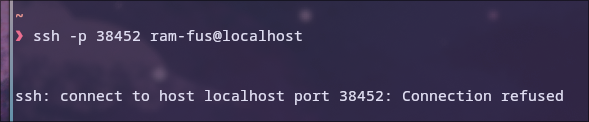
\includegraphics[scale=0.4]{images/loggingin-before-expsing-the-port.png}
	\caption{Connection refused}
\end{figure} 
To do this, we need to add a line to the Dockerfile and edit the docker run command.
\begin{lstlisting}[language=bash]
#add this with the port of your choice to the Dockerfile
EXPOSE 38452
#add -p to [p]ublish the desired port
docker run -d -p 38452 --name container -name
\end{lstlisting}
Even if we log in now, it still won't work because the user doesn't have a password.
\begin{figure}[h]
	\centering
	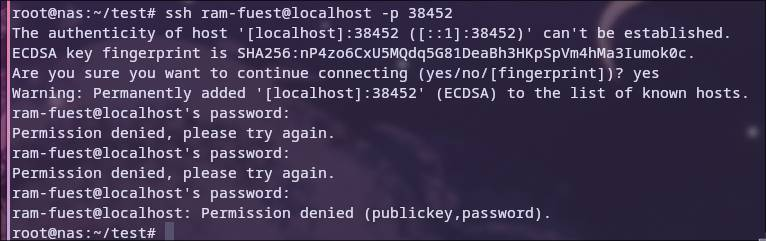
\includegraphics[scale=0.4]{images/failingtologin.png}
	\caption{Logging in without a password}
\end{figure} \\
To fix this we add this line to our Dockerfile:
\begin{lstlisting}[language=bash]
RUN echo 'root:youresecurepasswordhere' | chpasswd
\end{lstlisting}
We change the root password instead of the user password because we do not have \texttt{sudo} setup, and having to type sudo for every command when we are the only user is both unnecessary and annoying. 
\begin{figure}[h]
	\centering
	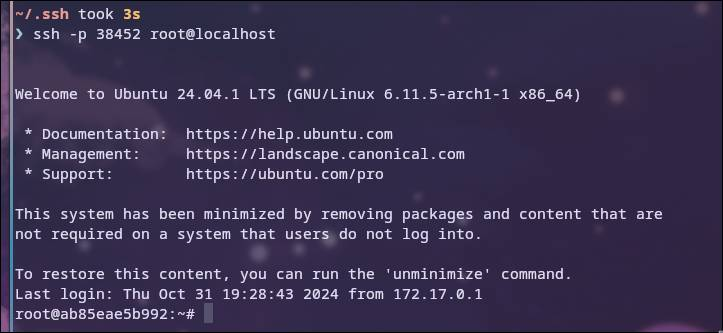
\includegraphics[scale=0.4]{images/workinglogin.png}
	\caption{working login}
\end{figure} \\
\newpage
\subsubsection{enabeling keypair authenthication}
To generate a key pair, we go back to our host system and run the command \texttt{ssh-keygen -b 4096} to generate a 4096-bit SSH key. \texttt{ssh-keygen}
On Linux, the keys are stored in the \texttt{~/.ssh} directory, but you can specify a location with \texttt{-f}. The file that ends with \texttt{.pub} is the public key, and the other is the private key.
\begin{figure}[h]
	\centering
	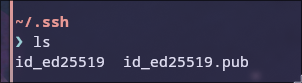
\includegraphics[scale=0.5]{images/keys-in-the-dir.png}
	\caption{keys in the directory}
\end{figure} \\
To copy the public key to the server we want to use it on, we use the command \texttt{ssh-copy-id} on Linux and \texttt{scp} on Windows and Mac. \texttt{ssh-copy-id}
\begin{figure}[h]
	\centering
	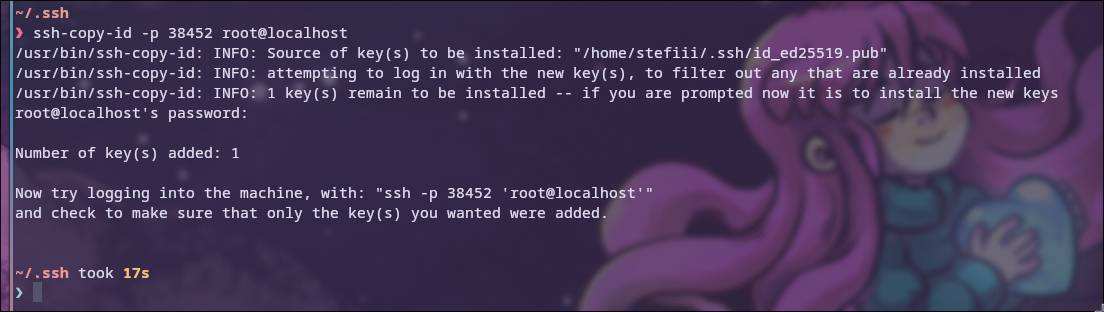
\includegraphics[scale=0.3]{images/ssh-copy-id.png}
	\caption{ssh-copy-id}
\end{figure} \\
After this we will not need to enter a password to authenticate.
\begin{figure}[h]
	\centering
	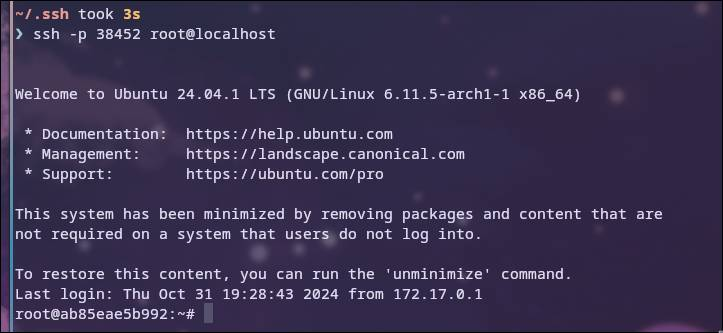
\includegraphics[scale=0.35]{images/login-with-key.png}
	\caption{logging with a key}
\end{figure} \\
\newpage
\subsubsection{Disable password authentication}
To only allow key authentication, we need to edit the \texttt{/etc/ssh/sshd\_config} file again.
To do this, we ssh into the server, open the file with a text editor of your choice, and edit this line.
\begin{lstlisting}[language=bash]
#change this
#PasswordAuthentication yes
#to this
PasswordAuthentication no
\end{lstlisting}
If we try to log in as another user for which we do not have a key, we cannot connect.
\begin{figure}[h]
	\centering
	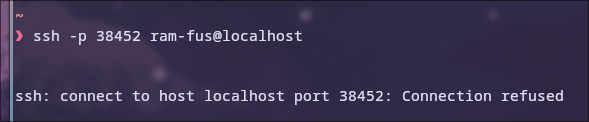
\includegraphics[scale=0.35]{images/nokey.png}
	\caption{Not having a key}
\end{figure} \\
\newpage
\bibliography{quellen}
\newpage
\section{List of figures}

\listoffigures
\newpage
\section{Attachments}
Dockerfile
\begin{lstlisting}[language=bash]
FROM ubuntu:latest

RUN apt update && apt upgrade -y &&\
    apt install iproute2 iputils-ping zsh net-tools vim -y
RUN ln -fs /usr/share/zoneinfo/Europe/Vienna /etc/localtime
RUN DEBIAN_FRONTEND=noninteractive apt install -y tzdata ssh
RUN echo 'root:password' | chpasswd
RUN sed -i 's/#Port 22/Port 38452/' /etc/ssh/sshd_config
RUN sed -i 's/#PermitRootLogin prohibit-password/PermitRootLogin yes/'\
    /etc/ssh/sshd_config
RUN groupadd -g 324 ram-Users &&\
    useradd -u 1024 ram-alois &&\
    useradd -u 1124 ram-berta &&\
    useradd -u 1224 ram-chris &&\
    useradd ram-fus &&\
    useradd ram-ram
RUN usermod -g ram-Users ram-alois &&\
    usermod -g ram-Users ram-berta
RUN usermod --shell /bin/bash ram-alois &&\ 
    usermod --shell /bin/bash ram-berta &&\
    usermod --shell /bin/zsh ram-chris 
RUN mkdir -p /data/fus &&\
    mkdir /data/fus/alois &&\
    mkdir /data/fus/berta &&\
    mkdir /data/fus/chris &&\
    mkdir /data/fus/public
RUN chgrp -R ram-Users /data/fus/ &&\
    chmod g+rw /data/fus/ &&\
    chown -R ram-alois:ram-Users /data/fus/alois/ &&\
    chmod -R u+wrx,g=r,o= /data/fus/alois/ &&\
    chown -R ram-berta:ram-Users /data/fus/berta/ &&\
    chmod -R u+wrx,g=r,o= /data/fus/berta/ &&\
    chown -R ram-chris:ram-Users /data/fus/chris/ &&\
    chmod -R u+wrx,g=,o= /data/fus/chris/ &&\ 
    chmod -R u+wrx,g+wrx,o=r /data/fus/public/
EXPOSE 38452
CMD service ssh start && tail -F /dev/null
\end{lstlisting}
alias.sh
\begin{lstlisting}[language=bash]
#!/bin/sh
alias relaunch="sudo sh -c 'docker stop itsi &&\
      docker rm itsi &&\
      docker buildx build -t itsi:latest . &&\
      docker run -d -p 38452:38452 --name itsi itsi:latest &&\
      docker exec -it itsi /bin/bash'"
alias rebuild="sudo sh -c 'docker buildx build -t itsi:latest . &&\
      docker run -d -p 38452:38452 --name itsi itsi:latest &&\
      docker exec -it itsi /bin/bash'"
alias stop="sudo sh -c 'docker stop itsi && docker rm itsi'"
\end{lstlisting}

\end{document}
